  % this file is called up by thesis.tex
% content in this file will be fed into the main document
% ----------------------- name of chapter  -------------------------
%\newgeometry{top=-0.4cm, left=0.9cm, right=1.5cm}
\chapter{Kinematic distributions in the Signal Regions}
\label{app:SRs}
% ----------------------- paths to graphics ------------------------

% change according to folder and file names
\ifpdf
\graphicspath{Appendices/AP5/figures/}
\else
\graphicspath{Appendices/AP5/figures/}
\fi
\vspace{-0.5cm}
This appendix shows some kinematic distributions in the Signal Regions:
\begin{itemize}
	\item SR1\tZc  (\Cref{app:SRs:SR1});
	\item SR2\tZc  (\Cref{app:SRs:SR2});
	\item SR3\tZc  using \DLrc (\Cref{app:SRs:SR3});
\end{itemize}

\newpage
%
%-------------------------------------------------------------------------------
\section{SR1\tZc}
\label{app:SRs:SR1}
\Cref{fig:sel:sr1:leps,fig:sel:sr1:jets} show the distributions 
of kinematic variables for events selected in the SR1\tZc.

\begin{figure}[!htbp]
	\centering
	\begin{tabular}{cc}
		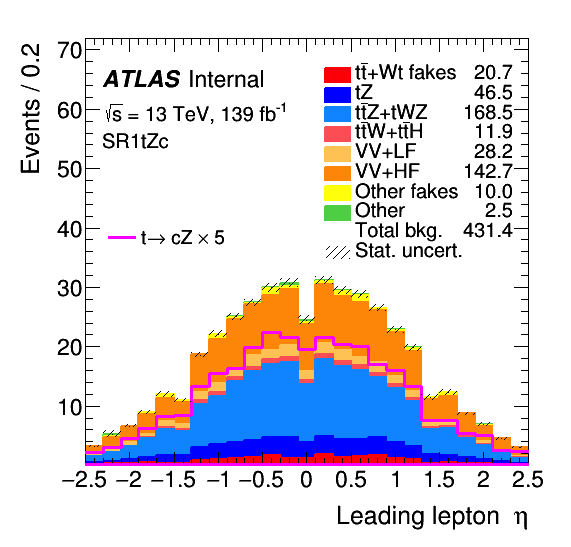
\includegraphics[width=.35\textwidth]{Appendices/AP5/figures/SR1/lep1_eta} &
		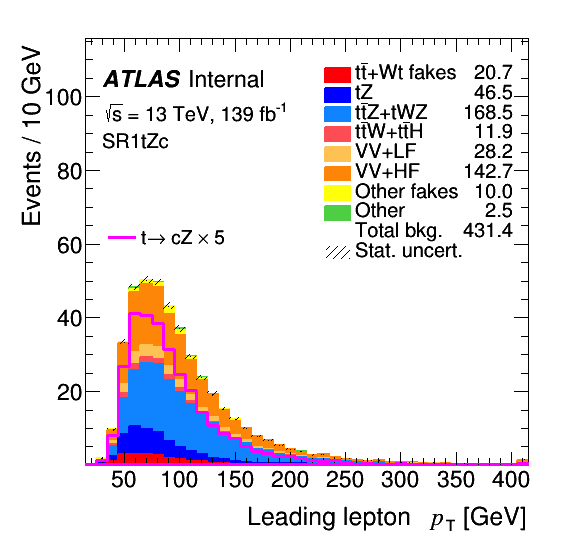
\includegraphics[width=.35\textwidth]{Appendices/AP5/figures/SR1/lep1_pt} \\
		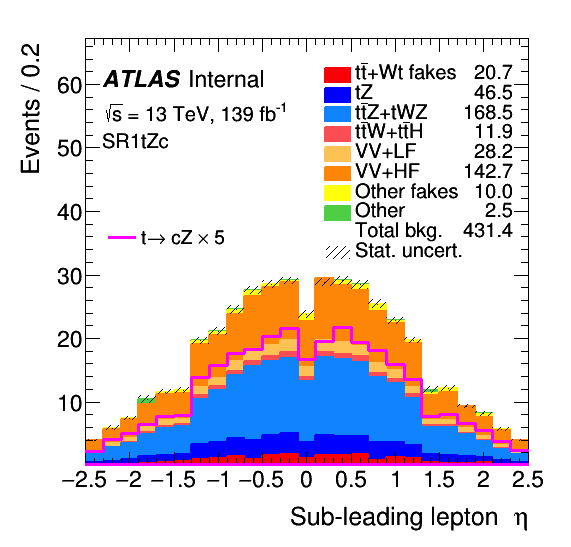
\includegraphics[width=.35\textwidth]{Appendices/AP5/figures/SR1/lep2_eta} &
		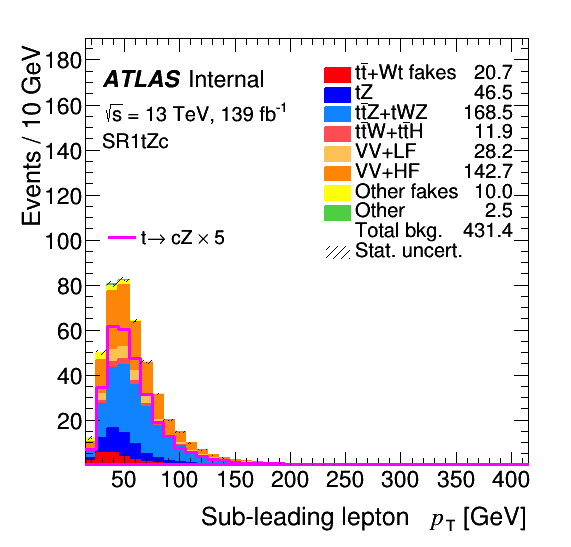
\includegraphics[width=.35\textwidth]{Appendices/AP5/figures/SR1/lep2_pt} \\
		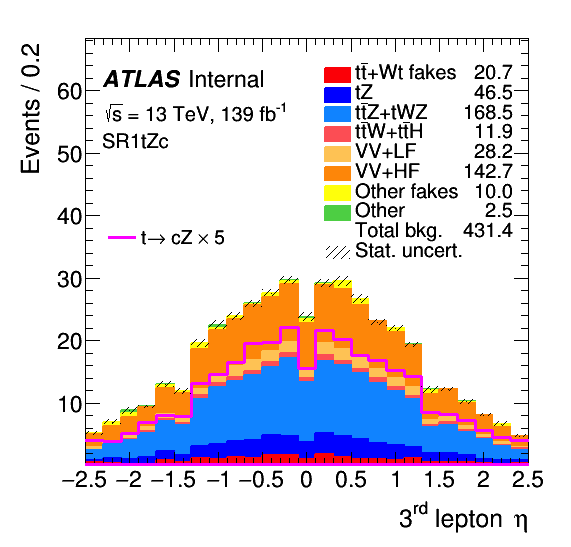
\includegraphics[width=.35\textwidth]{Appendices/AP5/figures/SR1/lep3_eta} &
		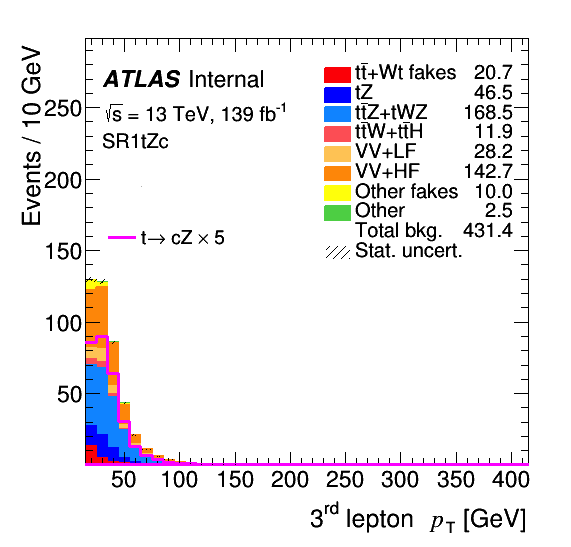
\includegraphics[width=.35\textwidth]{Appendices/AP5/figures/SR1/lep3_pt} \\
	\end{tabular}
	\caption{Pre-fit distributions of kinematic variables of leptons for events selected in the SR1\tZc.
		\ErrStatOnly
		\Blinded
	}%
	\label{fig:sel:sr1:leps}
\end{figure}

\begin{figure}[]
	\centering
	\begin{tabular}{cc}
		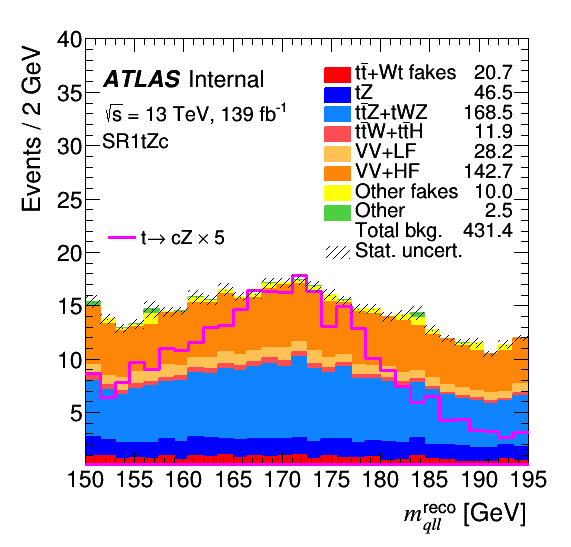
\includegraphics[width=.35\textwidth]{Appendices/AP5/figures/SR1/tFCNC} &
		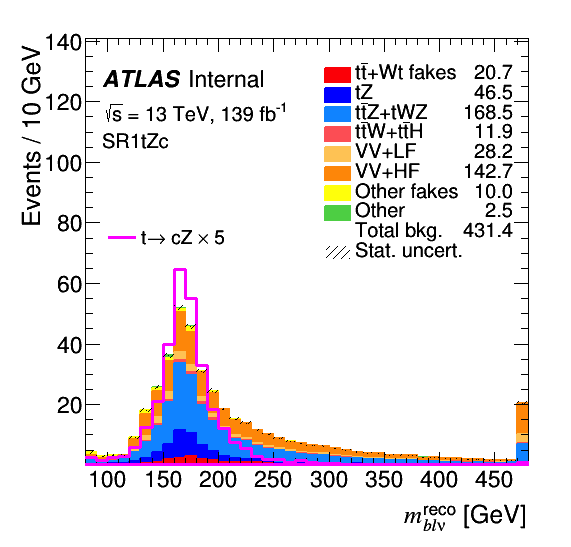
\includegraphics[width=.35\textwidth]{Appendices/AP5/figures/SR1/tSM} \\
		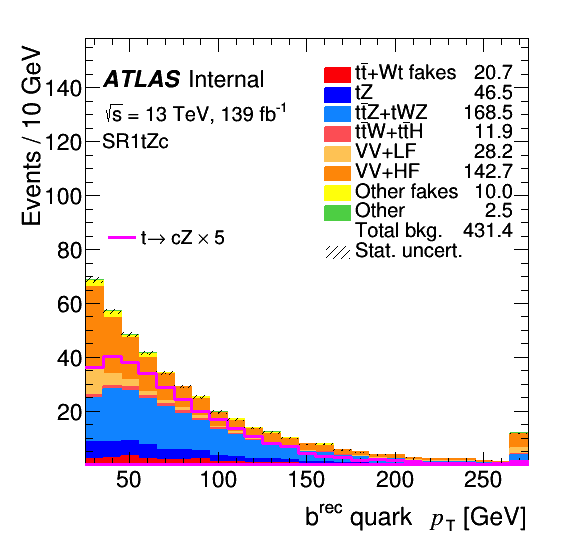
\includegraphics[width=.35\textwidth]{Appendices/AP5/figures/SR1/b_pt} & 
		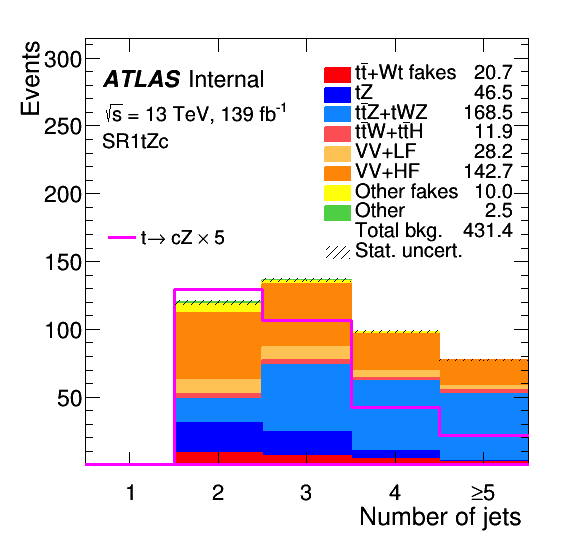
\includegraphics[width=.35\textwidth]{Appendices/AP5/figures/SR1/nJets} \\
	\end{tabular}
	\caption{Pre-fit distributions of kinematic variables of jets for events selected in the SR1\tZc.
		\ErrStatOnly
		\Blinded
	}%
	\label{fig:sel:sr1:jets}
\end{figure}

\clearpage
\FloatBarrier
\newpage
% -----------------------------------------------------------------------------
\section{SR2\tZc}
\label{app:SRs:SR2}
\Cref{fig:sel:sr2:leps,fig:sel:sr2:jets} show the distributions 
of kinematic variables for events selected in the SR1\tZc.

\begin{figure}[!htbp]
	\centering
	\begin{tabular}{cc}
		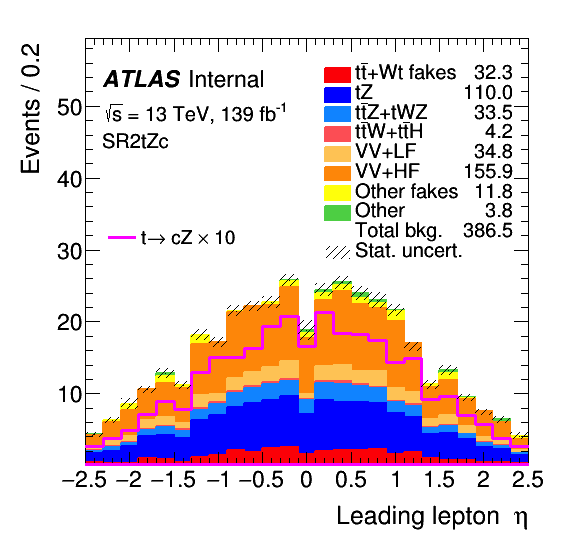
\includegraphics[width=.35\textwidth]{Appendices/AP5/figures/SR2/lep1_eta} &
		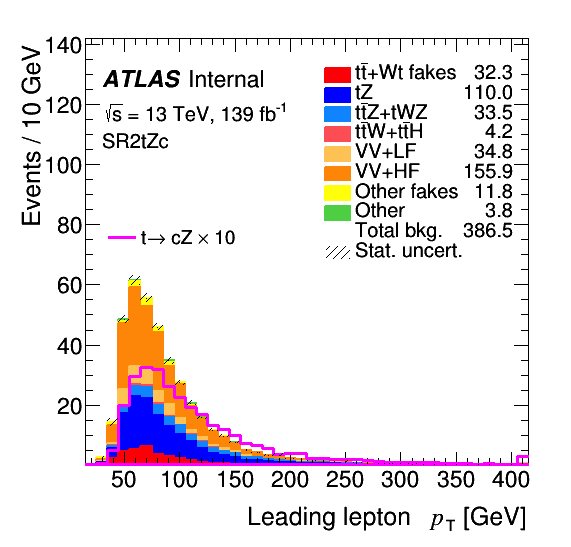
\includegraphics[width=.35\textwidth]{Appendices/AP5/figures/SR2/lep1_pt} \\
		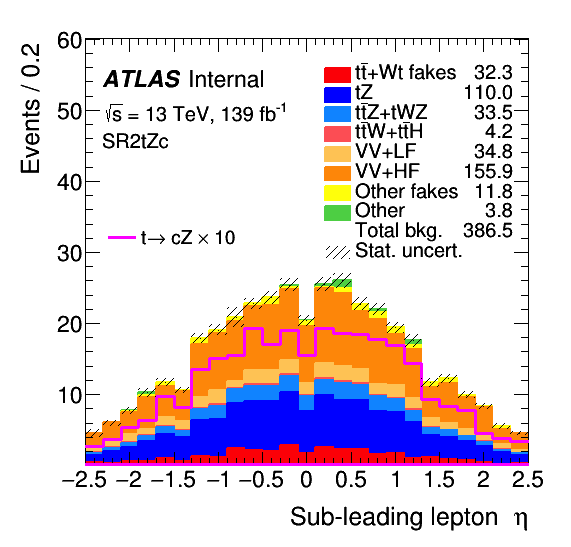
\includegraphics[width=.35\textwidth]{Appendices/AP5/figures/SR2/lep2_eta} &
		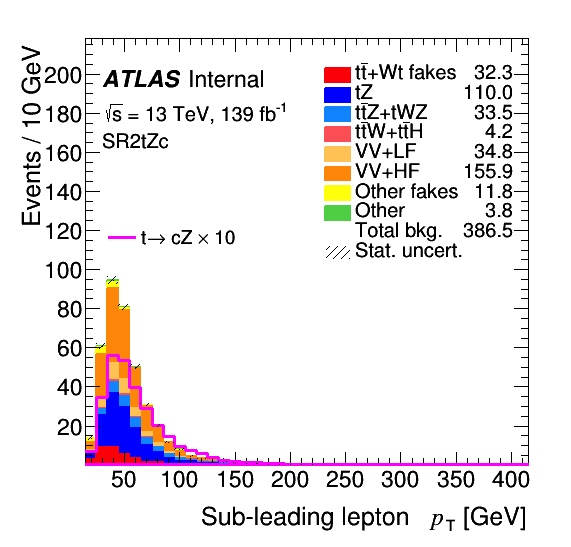
\includegraphics[width=.35\textwidth]{Appendices/AP5/figures/SR2/lep2_pt} \\
		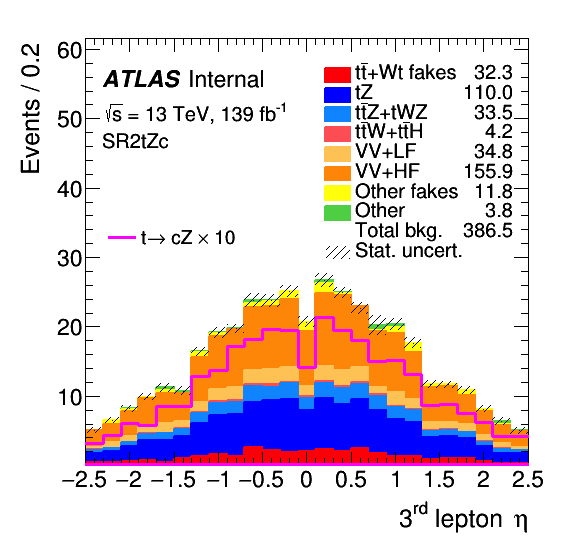
\includegraphics[width=.35\textwidth]{Appendices/AP5/figures/SR2/lep3_eta} &
		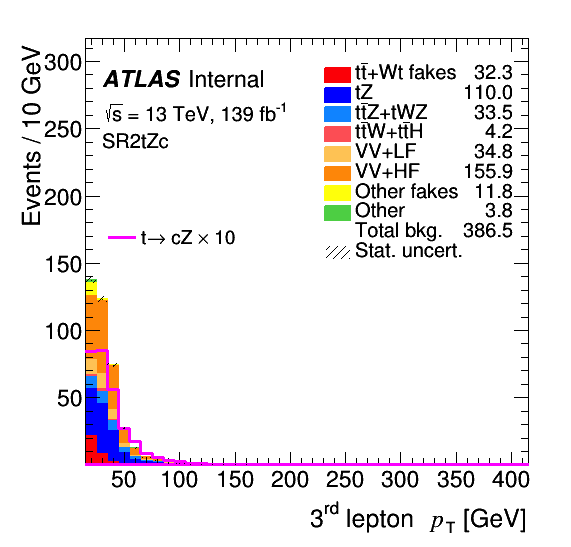
\includegraphics[width=.35\textwidth]{Appendices/AP5/figures/SR2/lep3_pt} \\
	\end{tabular}
	\caption{Pre-fit distributions of kinematic variables of leptons for events selected in the SR2\tZc.
		\ErrStatOnly
		\Blinded
	}%
	\label{fig:sel:sr2:leps}
\end{figure}

\begin{figure}[]
	\centering
	\begin{tabular}{cc}
		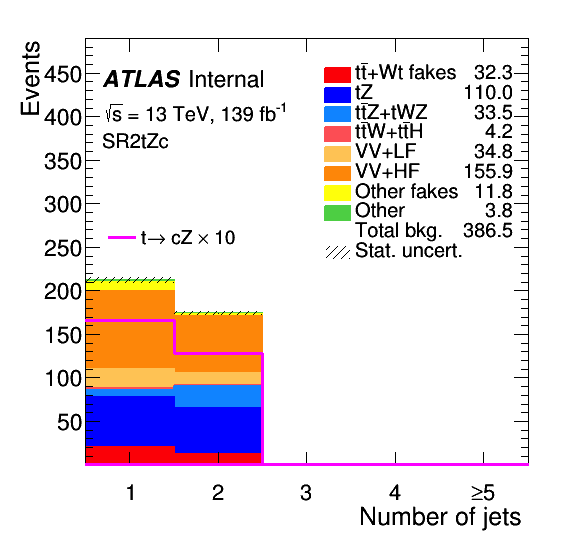
\includegraphics[width=.35\textwidth]{Appendices/AP5/figures/SR2/nJets} &
		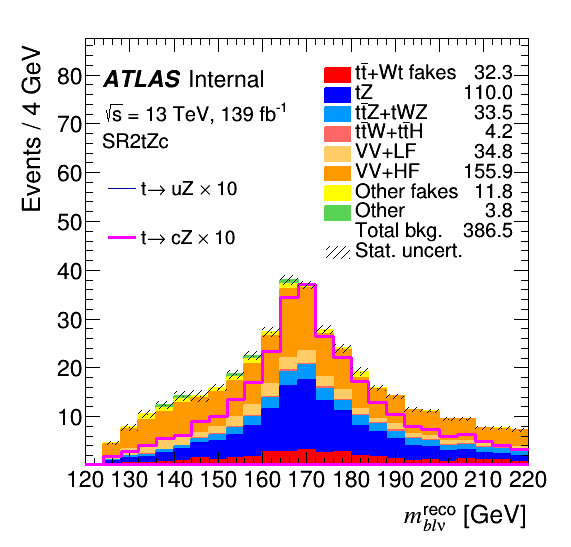
\includegraphics[width=.35\textwidth]{Appendices/AP5/figures/SR2/tSM} \\
		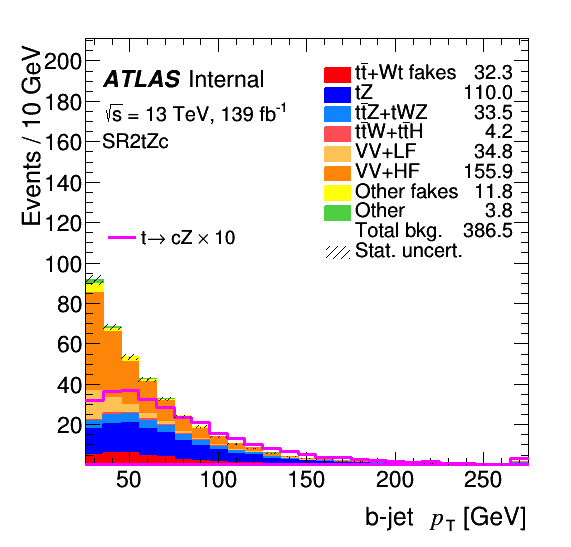
\includegraphics[width=.35\textwidth]{Appendices/AP5/figures/SR2/b_pt} & 
		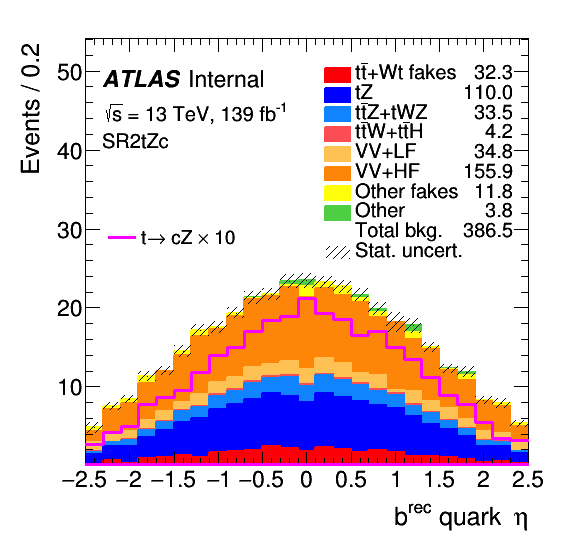
\includegraphics[width=.35\textwidth]{Appendices/AP5/figures/SR2/b_eta} \\
	\end{tabular}
	\caption{Pre-fit distributions of kinematic variables of jets for events selected in the SR2\tZc.
		\ErrStatOnly
		\Blinded
	}%
	\label{fig:sel:sr2:jets}
\end{figure}

\clearpage
\FloatBarrier
\newpage
% -----------------------------------------------------------------------------
\section{SR3\tZc}
\label{app:SRs:SR3}
\Cref{fig:sel:sr3:leps,fig:sel:sr3:jets} show the distributions 
of kinematic variables for events selected in the SR3\tZc.

\begin{figure}[!htbp]
	\centering
	\begin{tabular}{cc}
		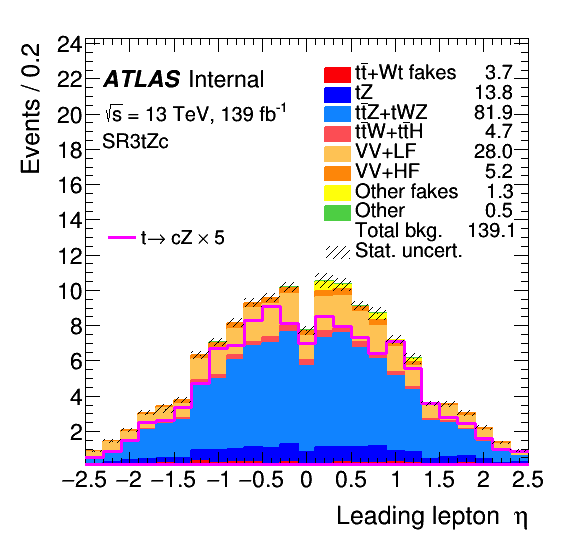
\includegraphics[width=.35\textwidth]{Appendices/AP5/figures/SR3_UsingDL1rc/lep1_eta} &
		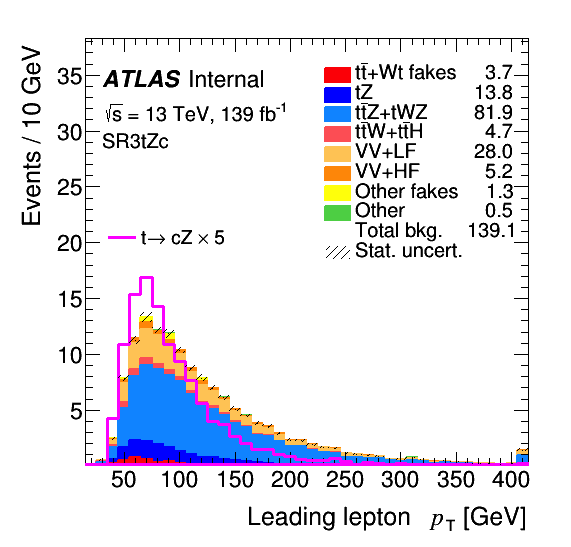
\includegraphics[width=.35\textwidth]{Appendices/AP5/figures/SR3_UsingDL1rc/lep1_pt} \\
		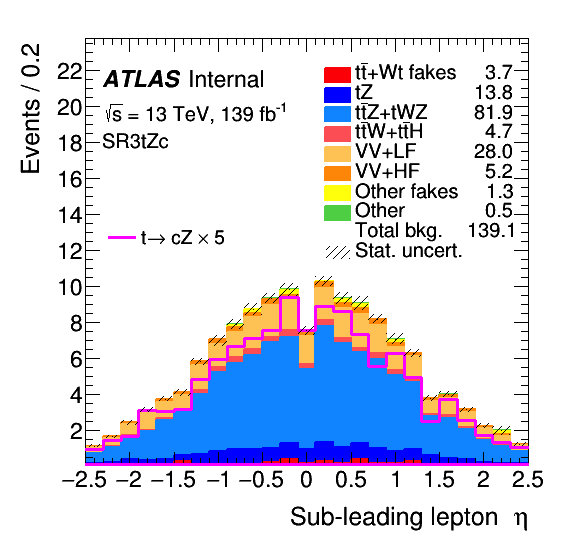
\includegraphics[width=.35\textwidth]{Appendices/AP5/figures/SR3_UsingDL1rc/lep2_eta} &
		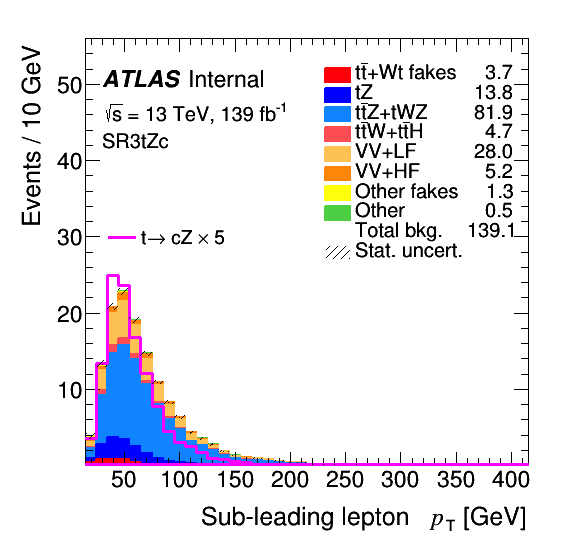
\includegraphics[width=.35\textwidth]{Appendices/AP5/figures/SR3_UsingDL1rc/lep2_pt} \\
		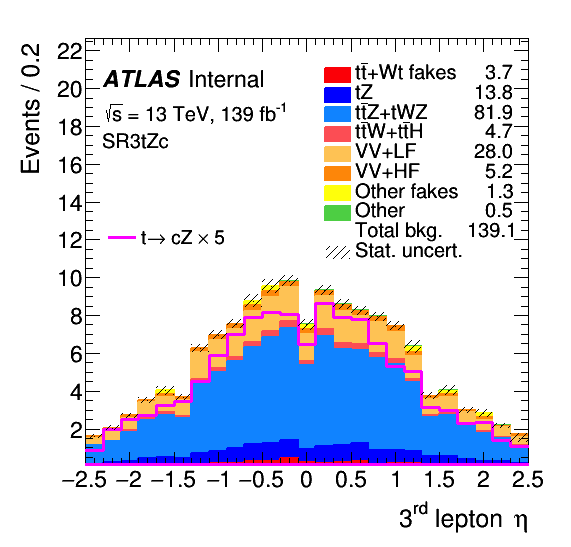
\includegraphics[width=.35\textwidth]{Appendices/AP5/figures/SR3_UsingDL1rc/lep3_eta} &
		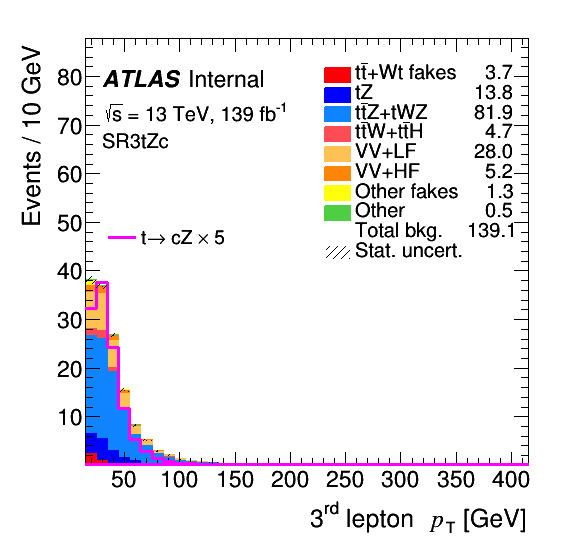
\includegraphics[width=.35\textwidth]{Appendices/AP5/figures/SR3_UsingDL1rc/lep3_pt} \\
	\end{tabular}
	\caption{Pre-fit distributions of kinematic variables of leptons for events selected in the SR3\tZc.
		\ErrStatOnly
		\Blinded
	}%
	\label{fig:sel:sr3:leps}
\end{figure}

\begin{figure}[]
	\centering
	\begin{tabular}{cc}
		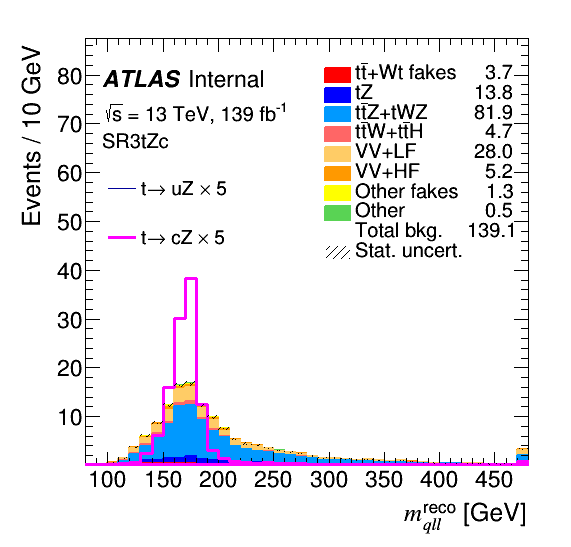
\includegraphics[width=.35\textwidth]{Appendices/AP5/figures/SR3_UsingDL1rc/tFCNC} &
		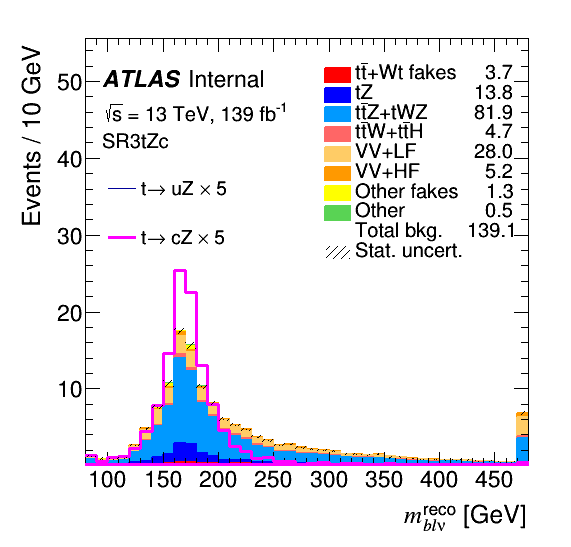
\includegraphics[width=.35\textwidth]{Appendices/AP5/figures/SR3_UsingDL1rc/tSM} \\
		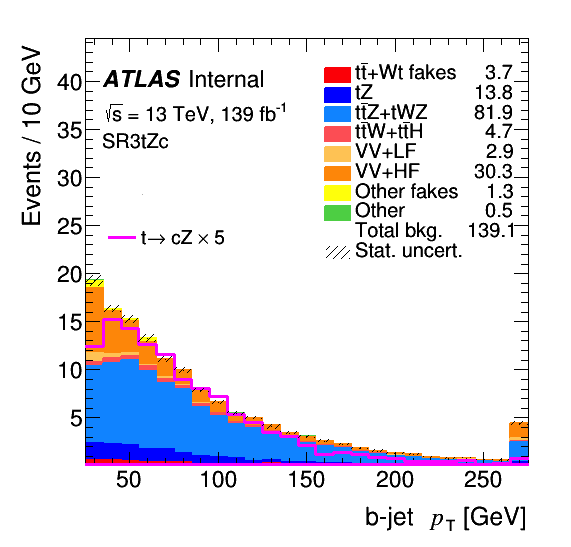
\includegraphics[width=.35\textwidth]{Appendices/AP5/figures/SR3_UsingDL1rc/b_pt} & 
		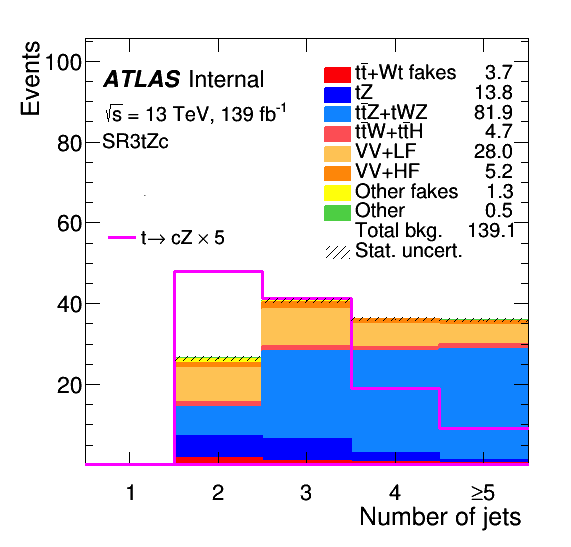
\includegraphics[width=.35\textwidth]{Appendices/AP5/figures/SR3_UsingDL1rc/nJets} \\
		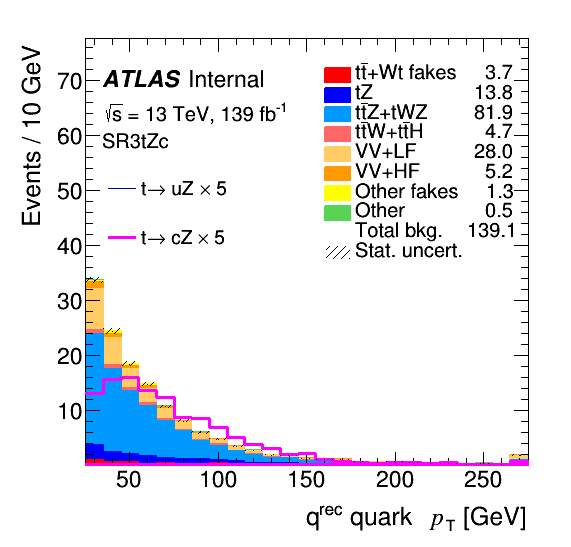
\includegraphics[width=.35\textwidth]{Appendices/AP5/figures/SR3_UsingDL1rc/q_pt}&
		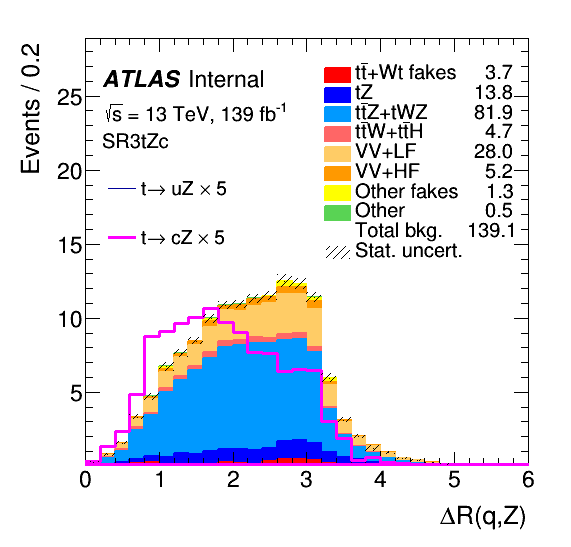
\includegraphics[width=.35\textwidth]{Appendices/AP5/figures/SR3_UsingDL1rc/qZ_dR} \\
	\end{tabular}
	\caption{Pre-fit distributions of kinematic variables of jets for events selected in the SR3\tZc.
		\ErrStatOnly
		\Blinded
	}%
	\label{fig:sel:sr3:jets}
\end{figure}

\clearpage
\FloatBarrier
% -----------------------------------------------------------------------------
